% This is an example manuscript for the SUNY Poly style options
%       sunypoly_ms.sty (Masters Thesis or Project)

\documentclass[letterpaper,11pt]{report}
\usepackage{sunypolyms}       % For Master's papers
\usepackage{ulem}       % underlining on style-page; see \normalem below
\usepackage{url}	% support for hyperlinks, especially in bibliography
\usepackage{pstricks}
\usepackage{epsfig}
\graphicspath{{./Figures/}} % This is the folder where figures are expected to go

% If this is a Master's project rather than a thesis, 
% uncomment this line.
%\isproject{true}

% Adjust placement of text frame to match your software and hardware.
% Usually 1.5in on left, 1in on right and bottom.  You may not need
% to uncomment this section.  Home printing systems are notorious for
% incorrectly placed margins due to paper loading and/or slipping
% problems
%
%\addtolength{\oddsidemargin}{.2in}
%    \setlength{\evensidemargin}{\oddsidemargin}
%\addtolength{\topmargin}{-.1in}


% May want theorems numbered by chapter
\newtheorem{theorem}{Theorem}[chapter]

% Put the title, author, and date in. 
\title{Sample Manuscript for the SUNY Poly Style Files}
\author{Your Name Here}
\date{May 9, 2021} % date is the date of graduation

% List previous degrees here, one \previousdegree for each degree.
%\previousdegree{M.A., University of Nebraska--Lincoln, 1984}
\previousdegree{B.S., SUNY Polytechnic Institute, 2019}

% Put the Thesis Adviser here. 
\advisor{Michael J. Reale}


% Put the committee here (including the advisor), one \professor for each. 
% The advisor must be SECOND!!!
\professor{Amos Confer\\
Associate Professor\\
Department of Computer \& Information Science}

\professor{Michael J. Reale, Chair\\
Associate Professor \\
Department of Computer \& Information Science}

\professor{Christopher Urban\\
Lecturer \\
Department of Computer \& Information Science}

% Information for style-page
% Note: Due to the way underlining is handled, any "extra" braces here will
% create a box which cannot be broken across lines. The \style argument below
% shows how emphasis should be done.

\style{Journal of Approximation Theory (together with the style known as
``sunypolyms'').  Bibliography follows van Leunen's {\it A} {\it Handbook}
{\it for} {\it Scholars}.}

\software{The document preparation package \TeX{} (specifically \LaTeX2e)
together with the style-file {\tt sunypolyms.sty}.}



\begin{document}

% Uncomment the "nocite" line to have all entries in your bibliography listed,
% regardless of whether they were cited.  This is often helpful in discovering
% you had not referenced a source you intended, especially if, like me,
% you add useful sources to your bibliography file as you discover them.  If
% you don't add sources to your bibliography until you write text that cites
% them, you may never need this line.
%
%\nocite{*}

\begin{romanpages}      % roman-numbered pages 
\ApprovalPage   % May comment-out until final version.
\TitlePage 
\CopyrightPage  % Should do nothing for Ph.D., if the degree is ever offered

% This should be a paragraph-style history of your academic work and
% industry efforts that may have contributed to your reaching this
% stage in your academic career.  
%
% Note that this is a special chapter style that must begin and end 
% the "vita" LaTeX environment.
%
\begin{vita}
An example of a vita:\\
William Confer began his career in the field of Computer Science early,
being exposed to programming in the early 1980's at home and at the
Classical Junior Academy of St. Louis, Missouri.  Upon completing 
the Computer Science program at Illinois College in 1999, William
worked as a software developer for the Department of Veteran Affairs,
Veteran Hospital Division and then moved south to Auburn, Alabama where he began his graduate career.
While at Auburn University, William has worked mostly in the fields of 
character recognition and wireless software development.  His efforts in
character recognition have culminated in this thesis work and a U.S. patent
he shares with his advisor, Richard Chapman.
\end{vita}


% This should be a very high level overview of the novel work presented
% in your manuscript.  Experiments should be outlined with the utmost brevity
% and only their most compelling results revealed.  Often the results
% identified here will lack numeric values which are saved for the Introduction
% chapter. 
%
% Note that this is a special chapter style that must begin and end 
% the "abstract" LaTeX environment.
%
\begin{abstract}
An example of an abstract:\\
This work presents an algorithm for on-line character recognition that is fast,
portable, and consumes very little memory for code or data.  The
algorithm is alphabet-independent, and does not require training
beyond entering the alphabet once. This algorithm uses a novel, parameter-based method
of feature extraction, \textit{activity}, to achieve high recognition 
accuracy.  Recognition accuracy is shown to be improvable dynamically without
further input from the user. The algorithm brings the capability to do
character recognition to classes of devices that heretofore have not
possessed that capability because of limited computing resources,
including mobile handsets, PDAs, pagers, toys, and other small devices. It
achieves recognition speeds of 16.8 characters per second on a 20MHz, 8-bit
microcontroller without floating-point.  The alphabet-independent
nature of the algorithm combined with its inherent resistance to regular noise interference
may allow it to enhance the capability of persons with impaired motor or nervous systems
to communicate with devices by writing or gesturing commands.  
Additionally, two human studies demonstrate the effectiveness of a simple,
activity-based recognizer for users of the stylized Graffiti alphabet and for
non-stylized variants of the English alphabet.  A final experiment shows how
recognition accuracy can be improved per user by modifying the parameters of
the activity metric over samples collected in the non-stylized study.

\end{abstract}



% Acknowledge and dedicate you work to whomever you wish.  It is common to
% identify those who significantly advised your work by name and at least 
% recognize your advisory committee as a whole.  This chapter is personal, 
% however, so a simple "R.I.P. Johhny Cash" is completely acceptable.
%
% Note that this is a special chapter style that must begin and end 
% the "acknowledgments" LaTeX environment.
%
\begin{acknowledgments}
An example of acknowledgments:\\
This work is dedicated to the memories of my grandmother, Lois Hoffman, and my 
truest friend, Jacob Palmatier.  Lois passed recently after a twenty-plus year battle
with multiple sclerosis.  She is the inspiration behind the majority of my work with 
character recognition.  Jacob was killed by a roadside bomb in Iraq while retrieving the mail.  He
was my only friend who didn't criticize pursuing higher degrees for all these years.
I miss each of them terribly.

I would like to thank each of my committee members, especially Richard Chapman,
and my outside reader, Chwan-Hwa Wu, for their support over the years.  
Jaun Gilbert supplied the tablet computers
used to collect samples for my final studies.  Gerry Dozier's assistance in evolutionary
techniques was crucial to the success of my attempts to optimize recognition.  Mike Spiegel,
an undergraduate student from Depauw University, was a tremendous help in organizing and collecting 
character samples.
I would also like to acknowledge the contributions of the following students for their assistance in the past:
Charlton Barker,
Tyson Begly,
David Boyette,
Barry Burton,
Crystal Collings,
Jim Han,
Travia Holder,
Kevin Jackson,
Justin Limbaugh,
Adam Luter,
Deitrick Mathews,
John Morley,
Christopher Nuby,
Marcus Parker,
and Bradley Scott.
An additional round of thanks go to
Auburn University Technology Transfer for assistance in acquiring the patent 
and in seeking licensees for activity-based recognizers.

This work was sponsored in part by the Auburn University Center for
Innovations in Mobile, Pervasive, Agile Computing Technologies
(IMPACT) and the U.S. Department of Education 
Graduate Assistance in Areas of National Need (GAANN) Fellowship. 

\end{acknowledgments}


\StylePage
\tableofcontents

% comment either of the following lines should your manuscript contain no 
% figures or tables
%
\listoffigures
\listoftables

\end{romanpages}        % All done with roman-numbered pages


\normalem       % Make italics the default for \em


% Introduction ((((( required! )))))
\chapter{Introduction}

In this section, you should talk about:
\begin{itemize}
    \item What problem you are trying to solve
    \item Why is it important
    \item Why is it challenging
\end{itemize}
You should also briefly summarize:
\begin{itemize}
    \item What your approach to the problem is
    \item Broadly what you accomplished
    \item Why your approach is novel
\end{itemize}

% Related work ((((( required! )))))
\chapter{Related Work}

Here you should summarize academic work that is related to the problem you are trying to solve. There are a few key points to this section:
\begin{enumerate}
    \item You need to properly cite works here, like this \cite{confer_2005_activity}.
    \item Your references should all be in the BibTeX format inside a .bib file.  You can do one of the following:
    \begin{itemize}
        \item Paste in the BibTeX citation of whatever work you are referring to (usually available in places like IEEE Xplore as "Cite This")
        \item Use a reference manager like Zotero or Mendeley, which allows exporting a .bib file
        \item Manually create the BibTeX entry, as shown in \cite{bibtexEntries}
    \end{itemize}
    \item Introduce each work by using the format shown (plus the citation):
    \begin{itemize}
        \item 1 author: "Confer \cite{confer_2005_activity} ... "
        \item 2 authors: "Eshelman and Schaffer \cite{eshelman93real} ..."
        \item 3 or more authors: "Kapsalisand et al. \cite{kapsalis93solving} ... "
    \end{itemize}
    \item At most, you should spend a paragraph on each work in question.  Consult your advisor for further specifications, but you should summarize:
    \begin{itemize}
        \item What is the core approach/idea
        \item What are its relevant results (if applicable)
        \item If possible, how the work is deficient (in particular if you are intending to address that deficiency)
    \end{itemize}
    \item \textbf{Your references should NOT be mostly composed of web links and/or online articles (e.g., Medium).}  Your Master's project/thesis is an academic work and should contain references to other peer-reviewed academic papers/journals/articles.
    \item Your references should be \textbf{recent, within 2 or at most 3 years}.  Some works you will cite will be seminal works that date further back, but in general you should be covering the state of the art.
    \item \textbf{Make sure you have sufficient references discussed here.}  It is not acceptable to discuss, say, 2 papers and think it is satisfactory coverage of the state of the art.
\end{enumerate}

\section{The Foobar Methods}

It is perfectly reasonable and encouraged to break up groups of methods into different subsections.  If you do so, introduce what is the unifying aspect of these approaches (e.g., "Some approach the problem by using the Foobar method").

\section{The Other Methods}

Here is where you would talk about these methods.

At the very end of this chapter, it is common to summarize what is overall missing in previous work that you specifically will address in your approach.

% Method 
%
\chapter{Method}

In this chapter, you should clearly discuss what your approach to solving the problem was.  Obviously, the contents of this section will vary significantly depending on the nature of the problem.  However, there are some common themes.

\section{Background}

Your target audience is someone with a computer science background who does not necessarily have specialization in your subarea (e.g., if your work is about machine learning, they may understand it in broad strokes, but may not know specifically what a neural network is or how it works).  This section is intended to provide enough background such that 1) your reader understands enough to understand your work and 2) you clearly understand your chosen area of interest.

\subsection{Project Writers}
While you should cite relevant software packages you utilize, the point of this section is NOT to explain the strengths/advantages of those software packages (e.g., do not give a summary of the virtues of NumPy \cite{harris2020array}).  Instead, you should focus on the underlying approaches that are directly and theoretically relevant to your work.  For example, if you use TensorFlow \cite{tensorflow2015-whitepaper} to build a Convolutional Neural Network (CNN), you should briefly discuss what a CNN is and how it works, not necessarily how TensorFlow the library works (unless, again, that is DIRECTLY relevant to your work, e.g., you have extended TensorFlow to optimize it).

\subsection{Thesis Writers}
Since you are writing a thesis, it is expected that your work has a strong mathematical and theoretical foundation to build upon.  Consequently, this section should contain sufficient mathematical background for the reader to understand your contribution.

\subsection{A Word on Diagrams, Figures, and Tables}
Diagrams and figures are welcome here, but there are a few things to note:
\begin{enumerate}
    \item All diagrams/figures/tables should have captions.
    \item Any diagram/figure from another source MUST cite their source in the caption.
    \item If you have a diagram, figure, or table, you MUST refer to it in-text and cite it using the \textbackslash ref command.  For example: ``See Figure \ref{LSTMExample} for an example of an LSTM network."
\end{enumerate}

\begin{figure}
\begin{center}
\includegraphics[height=0.50\textwidth]{lstm.png}
\end{center}
\caption{Example of LSTM Network \cite{lstmpaper}}
\label{LSTMExample}
\end{figure}

\subsubsection{A Further Word on Sub-Sub-Sections}
They exist.  Organize accordingly.

\section{Architecture/Structure}
Here you should describe the core of your approach.  In particular, you should describe what sets your approach apart from others.

In general, defer experiment-specific parameters until the "Experiments and Results" section.  Also, unless your work is specifically about generating data, defer discussions about datasets used until "Experiments and Results" as well.

Apart from small snippets, \textbf{you should NOT have your code copied and pasted into the body of this document}.  Your job here is describe in English what you have done; including most or all of your code is unhelpful and artificially inflates the size of the document. 




% Experiments and Results
%
\chapter{Experiments and Results}
This is where you specifically describe how you verified your work.  Some of these sections may be named slightly differently and/or have different contents, but the overall trend is the same.

\section{Data}
Where appropriate, you should have a section describing the dataset(s) you used.  Begin by describing the dataset as a whole, and then narrow down to what you did to the dataset before the experiments (e.g., number of subjects used, leave-one-out vs. 10-fold cross validation, etc.).  Feel free to split this discussion into subsections, such as "The Flintstone Dataset" and "Data Preparation".

\section{Parameters}
This section may be called "Training Parameters" or something similar, but describe the specific parameters of your experiments (e.g., how many epochs, batch size, learning rate, etc.).

\section{Results}
It is strongly recommended that you split this into different subsections if you have multiple sets of experiments you have tried.

Charts and figures are welcome, but in particular tables with results are critical.  See Table \ref{tbl_example} for an example of a table in \LaTeX.

Ideally, you should compare your results to that of the state of the art.  While success is not always guaranteed in research, at minimum you should be aware of how your work stacks up against that of other researchers.

\textbf{Discuss your results.}  Do not throw tables and numbers at the reader without some discussion of trends, positive points, negative points, etc.

\begin{table}
\begin{center}
\begin{tabular}{|c||c|c|c|}
\hline
Profile	&	Population Size	&	Aging Decay	&	Activity Regions	\\
\hline \hline 
A	&	40	&	0	&	Static	\\
B	&	40	&	0	&	Dynamic	\\
C	&	40	&	0.0001	&	Static	\\
D	&	40	&	0.0001	&	Dynamic	\\
\hline
E	&	30	&	0	&	Static	\\
F	&	30	&	0	&	Dynamic	\\
G	&	30	&	0.0001	&	Static	\\
H	&	30	&	0.0001	&	Dynamic	\\
\hline
I	&	20	&	0	&	Static	\\
J	&	20	&	0	&	Dynamic	\\
K	&	20	&	0.0001	&	Static	\\
L	&	20	&	0.0001	&	Dynamic	\\
\hline
M	&	10	&	0	&	Static	\\
N	&	10	&	0	&	Dynamic	\\
O	&	10	&	0.0001	&	Static	\\
P	&	10	&	0.0001	&	Dynamic	\\
\hline
Q	&	3	&	0	&	Static	\\
R	&	3	&	0	&	Dynamic	\\
S	&	3	&	0.0001	&	Static	\\
T	&	3	&	0.0001	&	Dynamic	\\
\hline
\end{tabular}
\caption{An example table from Dr. Confer's dissertation \cite{confer_2005_activity}}
\label{tbl_example}
\end{center}
\end{table}

% What aspects of the problem did you solve or not solve? ((((( !REQUIRED! ))))) 
% What are the anticipated benefits of this? ((((( !REQUIRED! ))))) 
%
\chapter{Conclusion}

Briefly summarize what you have actually accomplished in this work.  In particular:
\begin{itemize}
    \item What aspects of the problem did you solve or not solve?
    \item What are the anticipated benefits of this?
\end{itemize} 

% NEXT STEPS SHOULD SOMEONE CONTINUE THIS WORK ((((( required! )))))
%
\chapter{Future Work}
Here you should discuss what still remains to be completed and what you would work on if you were to continue.

\bibliographystyle{plain}
% change the following to whatever your .bib filename is (minus the ".bib")
\bibliography{myreferences}


\begin{appendix}
\chapter*{Appendices\addcontentsline{toc}{chapter}{Appendices}}
\begin{singlespace}

% You should have as many chapters as you need organized into separate files.
\chapter{Notes from the Original Style Files\label{appendix_notes}}

These style-files for use with \LaTeX{} are maintained by Darrel
Hankerson\footnote{Mathematics and Statistics, 221 Parker Hall,
844-3641, {\tt hankedr@auburn.edu}} and Ed
Slaminka\footnote{Mathematics and Statistics, 218 Parker,
{\tt slamiee@auburn.edu}}. 

In 1990, department heads and other representatives met with Dean Doorenbos
and Judy Bush-Crofton (then responsible for manuscript approval). This
meeting was prompted by a memorandum\footnote{Originally, the memorandum
was presented to Professor Larry Wit. A copy is available on request.} from
members of the mathematics departments concerning the {\em Thesis and
Dissertation Guide\/} and the approval process. There was wide agreement
among the participants (including Dean Doorenbos) to support the basic
recommendations outlined in the memorandum. The revised {\em Guide\/}
reflected some (but not all) of the agreements of the meeting.

Ms Bush-Crofton was supportive of the plan to obtain ``official approval''
of these style files.\footnote{Followup memoranda gave a definition of
``official approval.'' Copies will be sent on request.}  Unfortunately, Ms
Bush-Crofton left the Graduate School before the process was completed. In
1994, we were revisiting some of the same problems which were
resolved at the 1990 meeting.

In Summer 1994, I sent several memoranda to Ms Ilga Trend of the Graduate
School, reminding her of the agreements made at the 1990 meeting.
Professors A. Scottedward Hodel and Stan Reeves provided additional
support.  In short, it is essential that the Graduate School honor its
commitments of the 1990 meeting. It should be emphasized that Dean
Doorenbos is to thank for the success of that meeting.

Maintaining these \LaTeX{} files has been more work than expected, in
part due to continuing changes in requirement by the graduate school.
The Graduate School occasionally has complete memory loss about the
agreements of the 1990 meeting. If the Graduate School rejects your
manuscript based on items controlled by the style-files, ask
your advisor to contact the Graduate school (and copy to the chair) to urge
cooperation.

Finally, there have been several requests for additions to the package
(mostly formatting changes for figures, etc.). While such changes are not
really part of the thesis-style package, it could be beneficial to collect
these options and distribute with the package (making it easier on the next
student).  I'm especially interested in changes needed by various
departments.


%%%%%%%%%%%%%%%%%%%%%%%%%%%%%%%%%%%%%%%%%%%%%%%%%%%%%%%%%%%%%%%%%%%%
% REMOVE THIS SECTION WHEN PREPARING YOUR OWN MANUSCRIPT AND WRITE %
%          THE FILES NEEDED TO MEET THE ABOVE ORGANIZATION         % 
%%%%%%%%%%%%%%%%%%%%%%%%%%%%%%%%%%%%%%%%%%%%%%%%%%%%%%%%%%%%%%%%%%%%

\chapter{The SUNY Poly Style Guide Chapter Name is so\\ 
         Long we Break it Over Multiple Lines\label{second}}  % Use \\ for long titles 

\section{Help with \LaTeX{}}

Your choice to use \LaTeX{}, specifically \LaTeX2e{}, to typeset your thesis will almost certainly 
benefit your manuscript; not only in appearance, but in your ability to edit,
organize, reorganize, and direct the content without worry or delay because of formatting.  Whether 
you are new to \LaTeX{} or an experienced user, it never hurts to have a solid tool set and reference
materials to support your work.  

The standard books on the subject are Lamport's \emph{\LaTeX{}: A Document Preparation System}
\cite{lamport_1994_latex} and Hahn's \emph{\LaTeX{} for Everyone} \cite{hahn_1993_latex}.
These seminal texts can be found in almost any academic library, but are regularly put on
hold and not really up to date.  Several fine introductions and references are available on the
Internet.  My favorite is \emph{A Simplified Introduction to {\LaTeX}} \cite{greenberg_2006_latex}.
This free book is particularly valuable for understanding the bibliography tool, Bibtex, 
basic mathematics typesetting, and counters.  \emph{The Not so Short Introduction to \LaTeX2e{}}
\cite{oetiker_2008_latex} is an excellent mathematics typesetting reference, 
and \emph{Getting Started with \LaTeX{}} \cite{wilkins_1995_latex} gets you into the basics of
\LaTeX{} typesetting quickly.

\section{Overleaf}
I highly recommend the online \LaTeX{} editor Overleaf \cite{overleafRef}.  It vastly simplifies the process of editing \LaTeX{} documents without necessarily having to install software locally.

\section{Supporting tools}

Whenever I use \LaTeX to typeset a document, I seem to find myself using the same supporting tools
again and again.  This section identifies the most common of these tools
along with resources that can be used to get started or as a reference.

\subsection{Make}
I always use {\tt make} to build my multifile documents.
The {\tt Makefile} provided with this document provides, among
others, {\tt all}, {\tt clean}, {\tt clean\_tex}, {\tt clean\_code}, and {\tt code}
targets, but most commonly you will use the command
\begin{center}
{\tt make}
\end{center}

As you create any new \LaTeX{} files you should add them to the {\tt TEXFILES} variable
to ensure proper builds.  If you have any code that produces \LaTeX{} files, or files 
included by other \LaTeX{} files, you will need to manage that through the 
{\tt Makefile.code} file you create.

\subsection{Aspell}

\emph{Aspell} is the replacement for the \emph{ispell} command line spell checker.  
This tool is useful in it's ability to check spelling inside \TeX{} and \LaTeX{}
source files.  It provides a menu driven, interactive shell that is very simple to use.
To check the spelling of a file called ``{\tt myfile.tex}'', enter the command
\begin{center}
{\tt aspell -c myfile.tex}
\end{center}

\subsection{Gnuplot}

\emph{Gnuplot} is a data visualization tool that can produce very clear Extended Postscript (EPS)
graphics in 2D and 3D from mathematical expressions and data files.  While Gnuplot can export 
to many graphic formats, EPS is one of the most common used in \LaTeX{} documents because
of the simple use of the {\tt epsfig} package.  Figure \ref{fig_gnuplot} 
is an example Gnuplot graph from my dissertation added to the document with {\tt epsfig}.  

\begin{figure}
\begin{center}
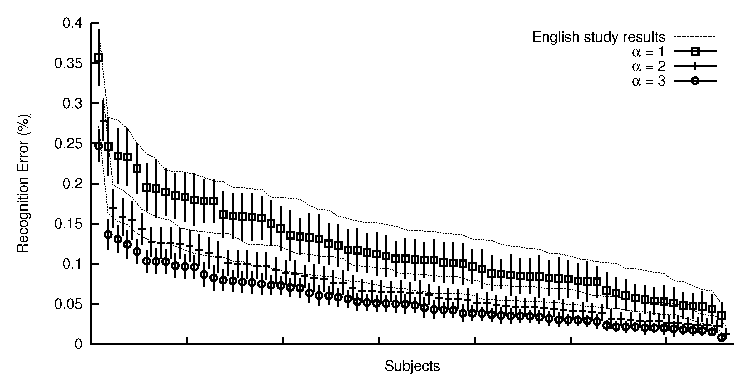
\epsfig{file=sample_gnuplot.eps, width=5in}
\caption{Example gnuplot graph included with the {\tt epsfig} package} 
\label{fig_gnuplot}
\end{center}
\end{figure}

%%%%%%%%%%%%%%%%%%%%%%%%%%%%%%%%%%%%%%%%%%%%%%%%%%%%%%%%%%%%%%%%%%%%
%                   STOP REMOVING HERE :-)                         %
%%%%%%%%%%%%%%%%%%%%%%%%%%%%%%%%%%%%%%%%%%%%%%%%%%%%%%%%%%%%%%%%%%%%





\end{singlespace}
\end{appendix}

\end{document}

